\documentclass[../generics]{subfiles}

\begin{document}

\chapter{Building Generic Signatures}\label{building generic signatures}

\index{generic signature}
\index{generic context}
\lettrine{B}{uilding a generic signature} from user-written requirements is an important topic which we have yet to cover. This bridges the gap between Chapter~\ref{generic declarations}, where we discussed the syntax for declaring generic parameters and stating requirements, and Chapter~\ref{genericsig}, which introduced generic signatures as semantic objects which collect the generic parameters and requirements of a generic declaration.

Unlike user-written requirements, the requirements of a generic signature are minimal, reduced, and appear in a certain order (we will see the formal definitions in Section~\ref{minimal requirements}). A fair amount of machinery is involved in building generic signatures. We're going to peel away the layers, starting from the entry points:
\begin{itemize}
\item All generic signatures are ultimately created by the \emph{primitive constructor}, which takes generic parameters and requirements known to already obey the necessary invariants.
\item The next code path concerns generic signatures of generic contexts. The \textbf{generic signature request} takes a generic context apart and delegates to the \textbf{inferred generic signature request}. The latter builds requirements from requirement representations with type resolution, hands the requirements to the minimization algorithm, and finally uses the primitive constructor to build the generic signature.
\item Another entry point exists to build a generic signature from scratch. The \textbf{abstract generic signature request} takes a list of requirements, hands the requirements off to the minimization algorithm, and again invokes the primitive constructor to build the generic signature.
\item For protocols, the \textbf{requirement signature request} solves the closely-related problem of building a requirement signature.
\end{itemize}

\paragraph{Primitive constructor}
\index{minimal requirement}%
\index{reduced requirement}%
\index{serialized module}%
\IndexDefinition{generic signature constructor}%
The primitive constructor is used directly when deserializing a generic signature, which was known to satisfy the invariants when it was serialized; or when the requirements are particularly trivial and the invariants hold by definition, such as the generic signature of a protocol, \verb|<Self where Self: P>|, or a generic signature with no requirements, like \verb|<A, B, C>|. In almost all other situations that call for building a generic signature ``from scratch,'' the \textbf{abstract generic signature request} should be used instead.

\paragraph{Generic signature request}
\index{request}%
\IndexDefinition{generic signature request}%
\index{request evaluator}%
\index{protocol declaration}%
\index{protocol extension}%
\Index{protocol Self type@protocol \texttt{Self} type}%
The generic signature of a generic context is constructed lazily by evaluating the \Request{generic signature request}. There are two easy cases to handle first:
\begin{itemize}
\item If the generic context is a protocol or an unconstrained protocol extension, the generic signature \verb|<Self where Self: P>| is built using the primitive constructor.

\Index{where clause@\texttt{where} clause}
\index{inheritance clause}
\index{generic parameter list}
\item If the generic context does not have a generic parameter list or trailing \texttt{where} clause of its own, it simply inherits the generic signature of the parent context. If the parent context is the top-level source file context, this is the empty generic signature. Otherwise, we recursively evaluate the generic signature request again, this time with the parent context.
\end{itemize}

\IndexDefinition{inferred generic signature request}
\index{request}
In all cases not covered by the two easy fallbacks above, the generic signature request actually has to do its work. It does this by kicking off the lower-level \Request{inferred generic signature request}, handing it a list of arguments:
\begin{enumerate}
\item The generic signature of the parent context, if any.
\item The current generic context's generic parameter list, if any.
\item The current generic context's trailing \texttt{where} clause, if any.
\item Any additional requirements to add.
\item A list of types eligible for requirement inference.
\item A flag indicating whether generic parameters can be subject to concrete same-type requirements.
\end{enumerate}

\paragraph{Inferred generic signature request} The name ``inferred generic signature request'' is a bit of a misnomer. Originally, it was named such because it performs requirement inference. The signature is not ``inferred'' in any sense.

\index{constrained extension}
\index{type resolution}
\index{requirement resolution}
\index{requirement inference}
A few words about some of the parameters above. At least one of the first two parameters must be specified; if there is no parent signature, and there are no generic parameters to add, the resulting generic signature is necessarily empty, which should have been handled already. The list of additional requirements (parameter 4) is only used for special inference behavior in extensions, described in Section~\ref{constrained extensions}. For all other declarations, the inferred generic signature request builds the list of requirements from syntactic representations, by resolving type representations in inheritance clauses and requirement representations in the \texttt{where} clause. If the generic context is a function or subscript declaration, the list of requirement inference sources (parameter 5) consists of the parameter and return types; otherwise, it is empty. The flag (parameter 6) enforces an artificial restriction whereby only certain kinds of declarations can constrain their innermost generic parameters to concrete types or other generic parameters. While it is generally useful to be able to write this,
\begin{Verbatim}
struct Outer<T> {
  func f() where T == Int {...}
}
\end{Verbatim}
or this,
\begin{Verbatim}
extension Outer where Element == Int {
  func f() {...}
}
\end{Verbatim}
something like the following is nonsensical and probably indicates a mistake on the user's part, because the innermost generic parameter \texttt{T} may as well be removed entirely, with all references to \texttt{T} replaced with \texttt{Int}:
\begin{Verbatim}
// error: same-type requirement makes generic parameter `T' non-generic
func add<T>(_ lhs: T, _ rhs: T) -> T where T == Int {
  return lhs + rhs
}
\end{Verbatim}

\begin{figure}\captionabove{Overview of the inferred generic signature request}\label{inferred generic signature request figure}
\begin{center}
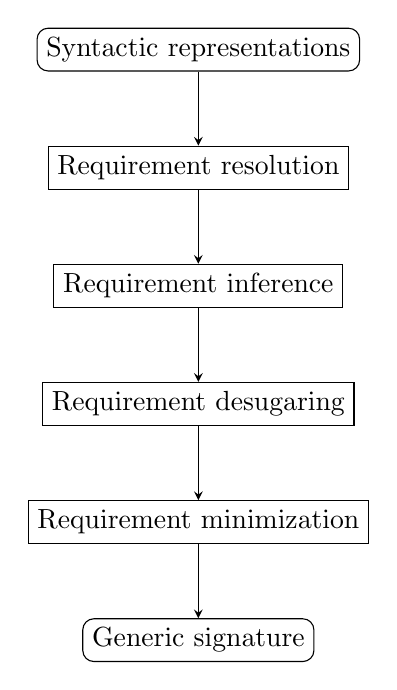
\begin{tikzpicture}[node distance=1.5cm]
\tikzstyle{data} = [rounded corners, draw=black, text centered]
\tikzstyle{stage} = [rectangle, draw=black, text centered]
\tikzstyle{arrow} = [->,>=stealth]

\node (SyntacticRepresentations) [data] {Syntactic representations};
\node (RequirementResolution) [stage, below of=SyntacticRepresentations] {Requirement resolution};
\node (RequirementInference) [stage, below of=RequirementResolution] {Requirement inference};
\node (RequirementDesugaring) [stage, below of=RequirementInference] {Requirement desugaring};
\node (RequirementMinimization) [stage, below of=RequirementDesugaring] {Requirement minimization};
\node (GenericSignature) [data, below of=RequirementMinimization] {Generic signature};

\draw [arrow] (SyntacticRepresentations) -- (RequirementResolution);
\draw [arrow] (RequirementResolution) -- (RequirementInference);
\draw [arrow] (RequirementInference) -- (RequirementDesugaring);
\draw [arrow] (RequirementDesugaring) -- (RequirementMinimization);
\draw [arrow] (RequirementMinimization) -- (GenericSignature);

\end{tikzpicture}
\end{center}
\end{figure}

With the various parameters at hand, the inferred generic signature request transforms arbitrary user-written requirements into minimal, reduced requirements via a multi-step process shown in Figure~\ref{inferred generic signature request figure}:
\begin{enumerate}
\item
\index{unbound dependent member type}%
\index{structural resolution stage}%
The first step is to construct a list of user-written requirements, resolving constraint types of generic parameter declarations and the requirement representations of the trailing \texttt{where} clause. This uses the structural resolution stage, meaning the resolved requirements might contain unbound dependent member types---they will be reduced to bound dependent member types before requirement minimization builds the final generic signature though.
\item Requirement inference (Section~\ref{requirementinference}) implements a heuristic for adding additional requirements which do not need to be explicitly stated for brevity.
\item Requirement desugaring (Section~\ref{requirement desugaring}) splits up conformance requirements where the constraint types are protocol composition types and parameterized protocol types, as well as certain forms of same-type requirements.
\item Requirement minimization is where the real magic happens; we will talk about the invariants established by this in Section~\ref{minimal requirements}, and pick up the topic again when we talk about the construction of a requirement machine from desugared requirements in Chapter \ref{rqm basic operation}.
\end{enumerate}

\IndexDefinition{conflicting requirement}%
\IndexDefinition{redundant requirement}%
\IndexFlag{warn-redundant-requirements}%
The inferred generic signature request emits diagnostics at the source location of the generic context in the following circumstances:
\begin{enumerate}
\item If the compiler is able to prove that no substitution map can ever simultaneously satisfy all of the requirements in the generic signature, the signature is said to contain \emph{conflicting requirements}. These will diagnose an error.
\item If some requirement can be shown to be a consequence of other requirements, the requirement is called a \emph{redundant requirement}. By default, redundant requirements are silently dropped, but if the \texttt{-Xfrontend -warn-redundant-requirements} flag is passed they are diagnosed as \index{warning}warnings.
\end{enumerate}

\begin{figure}\captionabove{Overview of the abstract generic signature request}\label{abstract generic signature request figure}
\begin{center}
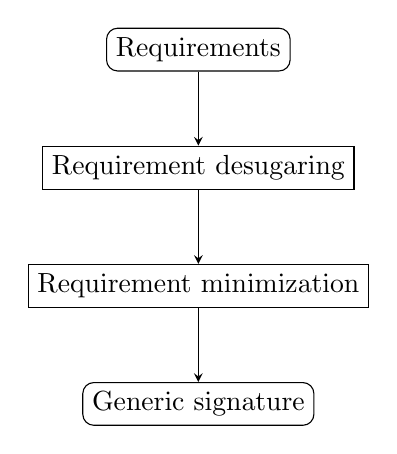
\begin{tikzpicture}[node distance=1.5cm]
\tikzstyle{data} = [rounded corners, draw=black, text centered]
\tikzstyle{stage} = [rectangle, draw=black, text centered]
\tikzstyle{arrow} = [->,>=stealth]

\node (Requirements) [data] {Requirements};
\node (RequirementDesugaring) [stage, below of=Requirements] {Requirement desugaring};
\node (RequirementMinimization) [stage, below of=RequirementDesugaring] {Requirement minimization};
\node (GenericSignature) [data, below of=RequirementMinimization] {Generic signature};

\draw [arrow] (Requirements) -- (RequirementDesugaring);
\draw [arrow] (RequirementDesugaring) -- (RequirementMinimization);
\draw [arrow] (RequirementMinimization) -- (GenericSignature);

\end{tikzpicture}
\end{center}
\end{figure}

\paragraph{Abstract generic signature request}
\IndexDefinition{abstract generic signature request}%
\index{request}%
\index{substituted requirement}%
This request builds a generic signature from a list of requirements that are not associated with a generic declaration or syntactic representations. The flow here is simpler, as shown in Figure~\ref{abstract generic signature request figure}. As input, it takes an optional parent generic signature, a list of generic parameter types to add, and a list of requirements to add.

At least one of the first two parameters must be specified; if there is no parent generic signature and there are no generic parameters to add, the result would be the empty generic signature, which the caller is expected to handle by not evaluating this request at all. The list of requirements to add is sometimes a list of substituted requirements, obtained by applying a substitution map to each requirement of some original generic signature. This will come up in Section~\ref{overridechecking} and Section~\ref{witnessthunksignature}.

\index{requirement inference}%
Like the inferred generic signature request, the abstract generic signature request does requirement desugaring and minimization. However, this request does not perform requirement inference, nor does it emit diagnostics, because there is no associated source location where to emit them.

\paragraph{Requirement signature request}
\index{request}%
\index{requirement signature}%
\IndexDefinition{requirement signature request}%
\IndexDefinition{structural requirements request}%
\IndexDefinition{type alias requirements request}%
\index{associated type declaration}%
\index{protocol declaration}%
\index{protocol type alias}%
\IndexDefinition{requirement signature constructor}%
This request builds a requirement signature from the protocol's requirements and type alias members, if any. It kicks off two other requests. The \Request{structural requirements request} collects user-written requirements from the protocol’s inheritance clause, associated type inheritance clauses, and \texttt{where} clauses on the protocol’s associated types and the protocol itself. The \Request{type alias requirements request} collects the protocol type aliases and converts them to same-type requirements. Finally, there is also a primitive constructor for building a requirement signature from a serialized representation, which bypasses requirement desugaring and minimization.

\paragraph{Protocol inheritance clauses}
\index{inheritance clause}
Recall from Section~\ref{protocols} that a constraint type written in a protocol's inheritance clause declares a conformance requirement with a subject type of \texttt{Self}. Qualified name lookup must be aware of protocol inheritance relationships, since a lookup into a protocol can also find members of inherited protocols. However, qualified lookup sits ``below'' generics. Building a protocol's requirement signature performs type resolution, which queries name lookup; those name lookups cannot in turn depend on the requirement signature having already been constructed. Thus, qualified name lookup can only look at syntactic constructs and cannot query the requirement signature.

The practical consequence of this design is that protocol inheritance must be explicitly stated, and cannot be implied as a non-trivial consequence of same-type requirements. After building a protocol's requirement signature, we ensure that any conformance requirements known to be satisfied by \texttt{Self} are actually explicit requirements written in the protocol's inheritance clause, or \texttt{where} clause entires with a subject type of \texttt{Self}. Anything else is diagnosed with a \index{warning}warning.

\begin{listing}\captionabove{Example showing non-obvious protocol inheritance relationship}\label{badinheritance}
\begin{Verbatim}
protocol Base {
  associatedtype Other: Base
  
  typealias Salary = Int
}

protocol Good: Base {
  typealias Income = Salary
}

// warning: protocol `Bad' should be declared to refine `Base' due to a
// same-type constraint on `Self'
protocol Bad {
  associatedtype Tricky: Base where Tricky.Other == Self
  
  typealias Income = Salary
  // error: cannot find type `Salary' in scope
}
\end{Verbatim}
\end{listing}
\begin{example}
In Listing~\ref{badinheritance}, the \texttt{Self} type of the \texttt{Bad} protocol is equivalent to the type parameter \texttt{Self.Tricky.Other} via a same-type requirement. The \texttt{Tricky} associated type conforms to \texttt{Base}, and the \texttt{Other} associated type of \texttt{Base} also conforms to \texttt{Base}. For this reason, the \texttt{Self} type of \texttt{Bad} actually conforms to \texttt{Base}.

However, this inheritance relationship is invisible to name lookup, so resolution of the underlying type of \texttt{Income} fails to find the declaration of \texttt{Salary}. After building the protocol's requirement signature, the type checker discovers the unexpected conformance requirement on \texttt{Self}, but at this stage, it is too late to attempt the failed name lookup again! The compiler instead emits a \index{warning}warning suggesting the user explicitly states the inheritance relationship in the declaration of \texttt{Bad}.
\end{example}

\section{Requirement Inference}\label{requirementinference}

\index{requirement}
\IndexDefinition{requirement inference}
\index{type resolution}
\index{generic arguments}
\index{interface resolution stage}
\index{structural resolution stage}
Requirement inference allows the user to omit any requirement that is implied by the application of a bound generic type to a generic argument. It is easiest to explain with an example. Recall that the standard library \texttt{Set} type declares a single \texttt{Element} generic parameter and requires that it conform to \texttt{Hashable}:
\begin{Verbatim}
struct Set<Element: Hashable> {...}
\end{Verbatim}
Say you're writing a function that returns returns a set of unique elements in a collection:
\begin{Verbatim}
func uniqueElements<S: Sequence>(_ seq: S) -> Set<S.Element> {...}
\end{Verbatim}
The type \verb|Set<S.Element>| only makes sense if \texttt{S.Element} conforms to \texttt{Hashable}. This is checked by type resolution in the interface resolution stage, after the generic signature has been built. However this requirement is not explicitly stated here. Instead, requirement inference \emph{adds} this requirement during the structural resolution stage when the generic signature is being built, ensuring that the type representation \verb|Set<S.Element>| can successfully resolve later.

You can always state an inferred requirement explicitly instead. Since this is useful for documentation purposes, the \verb|-warn-redundant-requirements| flag will not emit a \index{warning}warning if an explicit requirement is made redundant by an inferred requirement.
\begin{Verbatim}
func uniqueElements<S: Sequence>(_ seq: S) -> Set<S.Element>
    where S.Element: Hashable {...}
\end{Verbatim}

Requirement inference has an elegant formulation in terms of applying a substitution map to the requirements of a generic signature. In a sense, the problem being solved here is the opposite of checking generic arguments in type resolution (Section~\ref{checking generic arguments}). There, we determine if a substitution map satisfies the requirements of the referenced type declaration's generic signature, by applying the substitution map to each requirement and evaluating the truth of the substituted requirement. Requirement inference, on the other hand, \emph{adds} the substituted requirements to the generic signature being built, in order to \emph{make them true}.

In our example, we consider the type representation \texttt{Set<S.Element>} while building the generic signature of \texttt{uniqueElements()}. After resolving this to a type, we take its context substitution map, which has a single replacement type \texttt{S.Element}. Let's call this substitution map $\Sigma$:
\[\Sigma:=\SubstMapLongC{\SubstType{Element}{S.Element}}{\SubstConf{Element}{S.Element}{Hashable}}\]
Applying $\Sigma$ to both types in the requirement $\ConfReq{Element}{Hashable}$ of \texttt{Set}'s generic signature yields the substituted requirement $\ConfReq{S.Element}{Hashable}$, which is added to the list of desugared requirements which are fed into the minimization algorithm:
\[\ConfReq{Element}{Hashable}\otimes \Sigma = \ConfReq{S.Element}{Hashable}\]

\index{inheritance clause}
\index{generic parameter declaration}
\Index{where clause@\texttt{where} clause}
\index{underlying type}
\index{function declaration}
\index{subscript declaration}
\index{structural resolution stage}
\index{generic nominal type}
\index{type alias type}
\index{generic type alias}
Requirement inference considers type representations in the following positions when building the generic signature of a generic context:
\begin{enumerate}
\item The constraint types in inheritance clauses of generic parameter declarations.
\item Any types appearing inside the requirements of a \texttt{where} clause.
\item An additional list of type representations passed in to the inferred generic signature request. For functions and subscripts, this is the list of function parameter types together with the return type. For type aliases, this is the underlying type of the type alias.
\end{enumerate}
\index{substitution map}
\index{context substitution map}
Requirement inference resolves each of the above type representations in the structural type resolution stage (Chapter~\ref{typeresolution}), then recursively walks the type to find all generic nominal types and generic type alias types appearing within:
\begin{itemize}
\item Generic nominal types decompose into a nominal type declaration together with the context substitution map (Section~\ref{contextsubstmap}).
\item Type alias types decompose into a type alias declaration and a substitution map directly stored inside the type alias type (Section~\ref{more types}).
\end{itemize}
\index{substituted requirement}%
In both cases, we build a list of substituted requirements by applying the substitution map to each requirement of the type declaration's generic signature. These substituted requirements are precisely those that must become true in order for the type's generic arguments to satisfy the referenced type declaration's generic signature. Together with the user-written requirements, these substituted requirements form the basis for the generic signature being built. 
\begin{example}
The subject type of a substituted requirement need not be a type parameter. To help motivate the \emph{requirement desugaring} algorithm introduced in the next section, let's first define a generic struct with some non-trivial requirements:
\begin{Verbatim}
struct Transform<Key: Hashable, X: Sequence, Y: Sequence>
    where X.Element == Y.Element {}
\end{Verbatim}
Now, we're going to reference this struct from the type of a method parameter, which is one of the positions eligible for requirement inference:
\begin{Verbatim}
struct Transformer<E> {
  func transform<T: Hashable>(_: Transformer<Set<T>,
                                             Array<Array<E>>,
                                             Array<Array<Int>>) {}
}
\end{Verbatim}
The generic signature of \texttt{Transformer} has four requirements:
\begin{quote}
\begin{tabular}{lll}
\toprule
\textbf{Kind}&\textbf{Subject type}&\textbf{Constraint type}\\
\midrule
Conformance&\texttt{Key}&\texttt{Hashable}\\
Conformance&\texttt{X}&\texttt{Sequence}\\
Conformance&\texttt{Y}&\texttt{Sequence}\\
Same type&\texttt{X.[Sequence]Element}&\texttt{Y.[Sequence]Element}\\
\bottomrule
\end{tabular}
\end{quote}
The context substitution map of the function's parameter type is this:
\[
\SubstMapLongC{\SubstType{Key}{Set<T>}\\
\SubstType{X}{Array<Array<E>>}\\
\SubstType{Y}{Array<Array<Int>>}}{
\SubstConf{Key}{Set<T>}{Hashable}\\
\SubstConf{X}{Array<Array<E>>}{Sequence}\\
\SubstConf{Y}{Array<Array<Int>>}{Sequence}}
\]
Applying this substitution map to each requirement of the generic signature yields four substituted requirements:
\begin{quote}
\begin{tabular}{lll}
\toprule
\textbf{Kind}&\textbf{Subject type}&\textbf{Constraint type}\\
\midrule
Conformance&\texttt{Set<T>}&\texttt{Hashable}\\
Conformance&\texttt{Array<Array<E>>}&\texttt{Sequence}\\
Conformance&\texttt{Array<Array<Int>>}&\texttt{Sequence}\\
Same type&\texttt{Array<E>}&\texttt{Array<Int>}\\
\bottomrule
\end{tabular}
\end{quote}
Not all of these requirements are useful. The first three are conformance requirements with a concrete subject type, so they are discarded by requirement desugaring after they are checked to be satisfied. The fourth substituted requirement states that the two array types \texttt{Array<E>} and \texttt{Array<Int>} are the same type. Requirement desugaring replaces this requirement with the simpler equivalent requirement $\FormalReq{E}{Int}$.

In the end, the generic signature of \texttt{Transformer.transform()} becomes the following:
\begin{quote}
\begin{verbatim}
<E, T where T: Hashable, E == Int>
\end{verbatim}
\end{quote}
The \verb|T: Hashable| requirement was explicitly stated, while the $\FormalReq{E == Int}$ requirement was inferred.
\end{example}
\index{generic type alias}
\begin{example}
Requirement inference is specifically defined to look at type alias types, making the building of generic signatures one of a handful of places in the language where writing a sugared type has a semantic effect. Consider this example:
\begin{Verbatim}
typealias EquatableArray<Element> = Array<Element>
    where Element: Equatable

func allEqual<Element>(_: EquatableArray<Element>) -> Bool {}
\end{Verbatim}
The \texttt{allEqual()} function has a single \texttt{Element} generic parameter, and a parameter of type \texttt{EquatableArray<Element>}. The \texttt{EquatableArray} generic type alias requires that its generic parameter is \texttt{Equatable}. Thus, the generic signature of \texttt{allEqual()} contains a single requirement introduced by requirement inference:
\begin{quote}
\begin{verbatim}
<Element where Element: Equatable>
\end{verbatim}
\end{quote}

Suppose we wrote our function without reference to the type alias:
\begin{Verbatim}
func allEqual<Element>(_: Array<Element>) -> Bool {}
\end{Verbatim}
Now there is nothing for requirement inference to do, and \texttt{allEqual()} receives a different generic signature with no requirements:
\begin{quote}
\begin{verbatim}
<Element>
\end{verbatim}
\end{quote}
\end{example}

\index{parameterized protocol type}
\begin{example}
The underlying type of a type alias need not mention the generic parameter types of the type alias at all. Before parameterized protocol types were added to the language, a few people discovered a funny trick that could be used to simulate them:
\begin{Verbatim}
typealias SequenceOf<T, E> = Any where T: Sequence, T.Element == E

func sum<S: SequenceOf<S, Int>>(_: T) {...}
\end{Verbatim}
To understand what this does, and how, consider the generic signature of \texttt{SequenceOf}:
\begin{quote}
\begin{verbatim}
<T, E where T: Sequence, E == T.[Sequence]Element>
\end{verbatim}
\end{quote}
This signature has two requirements:
\begin{quote}
\begin{tabular}{lll}
\toprule
\textbf{Kind}&\textbf{Subject type}&\textbf{Constraint type}\\
\midrule
Conformance&\texttt{T}&\texttt{Sequence}\\
Same type&\texttt{E}&\texttt{T.[Sequence]Element}\\
\bottomrule
\end{tabular}
\end{quote}
The \texttt{sum()} function declares a generic parameter \texttt{S} with the type \texttt{SequenceOf<S, Int>} in its inheritance clause. The underlying type of this type alias is \texttt{Any}, so the inheritance clause introduces the trivial requirement $\ConfReq{S}{Any}$. However, requirement inference also visits the type \texttt{SequenceOf<S, Int>} in the inheritance clause. This type alias type has the following substitution map:
\[
\SubstMapC{
\SubstType{T}{S},\,\SubstType{E}{Int}
}{\SubstConf{T}{S}{Sequence}}
\]
Applying this substitution map to each requirement in the type alias declaration's generic signature yields the following two substituted requirements:
\begin{quote}
\begin{tabular}{lll}
\toprule
\textbf{Kind}&\textbf{Subject type}&\textbf{Constraint type}\\
\midrule
Conformance&\texttt{S}&\texttt{Sequence}\\
Same type&\texttt{Int}&\texttt{S.[Sequence]Element}\\
\bottomrule
\end{tabular}
\end{quote}
So the generic signature of \texttt{sum()} becomes the following:
\begin{quote}
\begin{verbatim}
<S where S: Sequence, S.[Sequence]Element == Int>
\end{verbatim}
\end{quote}
Indeed, our function \texttt{sum()} could have been written as follows:
\begin{Verbatim}
func sum<S>(_: T) where S: Sequence, S.Element == Int {...}
\end{Verbatim}
Which is of course equivalent to the modern syntax:
\begin{Verbatim}
func sum<S>(_: T) where S: Sequence<Int> {...}
\end{Verbatim}
\end{example}

\index{generic arguments}
\index{interface resolution stage}
\begin{example}
It is instructive to consider the behavior of type resolution's generic argument checking, with and without requirement inference. Requirement inference only happens if a new generic signature actually needs to be built, either because the generic context adds generic parameters or has a trailing \texttt{where} clause. However, if neither is present, the generic context always inherits the generic signature from its parent context, without giving requirement inference the opportunity to introduce requirements.

Consider the below generic struct type containing three functions:
\begin{Verbatim}
struct G<T, U> {
  func example1<V>(_: V, _: Set<T>) {}  // infers T: Hashable
  func example2(_: Set<T>) where U: Sequence {}  // infers T: Hashable
  func example3(_: Set<T>) {}  // nothing inferred; error diagnosed
}
\end{Verbatim}
\begin{enumerate}
\item The first function declares a generic parameter list, so the inferred generic signature request runs. Requirement inference adds the inferred requirement $\FormalReq{T}{Hashable}$; thus the generic signature is
\begin{quote}
\begin{verbatim}
<T, U, V where T: Hashable>
\end{verbatim}
\end{quote}
Type resolution then checks the generic arguments of \texttt{Set<T>} in the interface resolution stage. The generic argument \texttt{T} is mapped into the function's generic environment, producing the archetype $\archetype{T}$. The substituted requirement $\Conf{\archetype{T}}{Hashable}$ is satisfied, because $\archetype{T}$ conforms to \texttt{Hashable}.

\item In the second example, the generic signature is slightly different, but the generic argument check succeeds for the same reason:
\begin{quote}
\begin{verbatim}
<T, U where T: Hashable, U: Sequence>
\end{verbatim}
\end{quote}

\item In the third example, the declaration does not have a generic parameter list or \texttt{where} clause, so it inherits the generic signature from the parent context, \texttt{<T, U>}. In this generic environment, the archetype $\archetype{T}$ does not conform to \texttt{Hashable}, so the type representation \texttt{Set<T>} cannot be resolved. An error is diagnosed, pointing at the source location of the type representation.
\end{enumerate}
\end{example}

\paragraph{Requirement signatures}
\index{requirement signature request}
\index{limitation}
\index{protocol dependency graph}
Unlike the inferred generic signature request, the requirement signature request does not perform requirement inference. Originally the reasoning was that all requirements imposed on the concrete conforming type should be explicitly stated inside the protocol body, for clarity.

\index{protocol dependency graph}
\index{associated conformance requirement}
This has since been retconned\footnote{``revise (an aspect of a fictional work) retrospectively, typically by introducing a piece of new information that imposes a different interpretation on previously described events.''} into an appeal for implementation simplicity. For various reasons, when computing the requirement signature of a protocol we need to construct something called the \emph{protocol dependency graph} very early. This graph, which you will meet in Section~\ref{recursive conformances}, records the relationship between a protocol and other protocols it references from the right hand side of associated conformance requirements. Since requirement inference can introduce new conformance requirements, it is incompatible with protocol requirement signature minimization.

For example, the $\ConfReq{Particle}{Hashable}$ requirement cannot 
be omitted below, because the type \texttt{Set<Particle>} would no longer satisfy \texttt{Set}'s $\ConfReq{Element}{Hashable}$ requirement:
\begin{Verbatim}
protocol Cloud {
  associatedtype Particle: Hashable
  associatedtype Particles: Sequence
      where Particles.Element == Set<Particle>
}
\end{Verbatim}

\section{Requirement Desugaring}\label{requirement desugaring}

After requirement resolution and requirement inference, the inferred generic signature request has collected a list of requirements, which together with the requirements in the parent generic signature, form the basis for a new generic signature. (The abstract generic signature request \emph{starts} here; the list of requirements are directly provided by the caller, rather than being constructed from user-written requirement representations and requirement inference.)

There are several extra steps before we can arrive at the \emph{minimal}, \emph{reduced} list of requirements that appear in the final generic signature. The first step is \emph{requirement desugaring}, which establishes the invariants defined below. These invariants will become important when we build rewrite rules from requirements in Section~\ref{building rules}.
\IndexDefinition{desugared requirement}
\index{requirement desugaring|see {desugared requirement}}
\begin{definition}\label{desugaredrequirementdef} A \emph{desugared requirement} satisfies two conditions:
\begin{enumerate}
\item If the requirement is a conformance requirement, the constraint type must be a protocol type (and not a protocol composition or parameterized protocol).
\item The subject type must be a type parameter.
\end{enumerate}
\end{definition}

\index{conformance requirement}
\index{protocol type}
\index{protocol composition type}
\index{parameterized protocol type}
The idea behind establishing the first invariant was already introduced informally in Sections~\ref{constraints} and Section~\ref{protocols}. Now we will see the precise semantics in the form of an algorithm.

\index{protocol substitution map}
\index{primary associated type}
\index{same-type requirement}
\begin{algorithm}[Expanding conformance requirements]\label{expand conformance req algorithm} Takes a list of conformance requirements as input. Outputs a new list of equivalent requirements where all conformance requirements have a protocol type on the right hand side.
\begin{enumerate}
\item Initialize the output list to an empty list.
\item Initialize the worklist with all conformance requirements from the input list.
\item (Check) If the worklist is empty, return the output list.
\item (Loop) Take a conformance requirement $\texttt{T}:~\texttt{C}$ from the worklist.
\item (Base case) If \texttt{C} is a protocol type, add this conformance requirement \texttt{T:~C} to the output list.
\item (Composition) If \texttt{C} is a protocol composition type, visit each protocol composition member $\texttt{M}\in\texttt{C}$. If \texttt{M} is a class type or \texttt{AnyObject}, add the superclass or layout requirement \texttt{T:~M} to the output list. Otherwise, \texttt{M} might need to be decomposed further, so add a conformance requirement \texttt{T:~M} to the worklist.
\item (Parameterized) If \texttt{C} is a parameterized protocol type \texttt{P<G1, ..., Gn>} with base type \texttt{P} and generic arguments \texttt{Gi}, decompose the requirement as follows:
\begin{enumerate}
\item The base type \texttt{P} is always a protocol type. Add the conformance requirement \texttt{T:~P} to the output list.
\item For each primary associated type \texttt{Ai} of \texttt{P}, construct the protocol substitution map for the subject type \texttt{T}, and apply it to the declared interface type of \texttt{A}:
\[\texttt{Self.[P]Ai} \otimes \SubstMapLongC{\SubstType{Self}{T}}{\SubstConf{Self}{T}{P}} = \texttt{T.[P]Ai}\]
(Note that if \texttt{T} is a type parameter, the substituted type is the dependent member type \texttt{T.[P]Ai}; however, \texttt{T} might also be a concrete type, in which case we look up the type witness of \texttt{Ai} in the conformance $\ConfReq{T}{P}$.)

Add the same-type requirement $\FormalReq{T.[P]Ai == Gi}$ to the output list.
\end{enumerate}
\end{enumerate}
\end{algorithm}
This gives us the first invariant of Definition~\ref{desugaredrequirementdef}. To understand how requirement desugaring establishes the second invariant, we need to understand what it means for a requirement to have a concrete subject type. Requirements involving concrete types can appear when building a new generic signature from substituted requirements obtained by applying a substitution map to the requirements of a different generic signature. We already saw how this can happen with requirement inference, and it will come up again in Section~\ref{overridechecking} and Section~\ref{witnessthunksignature}.

\index{global conformance lookup}
Recall from Section~\ref{checking generic arguments} that a requirement where all types are fully concrete is a ``statement'' whose truth can be evaluated. A conformance requirement with a concrete subject type can be checked by performing a global conformance lookup; a same-type requirement between concrete types can be checked by comparing two types for canonical equality, and so on.

\index{conflicting requirement}
\index{redundant requirement}
If a requirement with a concrete subject type is satisfied, the requirement is necessarily redundant because it does not give us any new information about the generic signature's type parameters. If it is unsatisfied, the requirement is a conflicting requirement; an error is diagnosed.

\begin{example}
The requirement \texttt{Int:\ Hashable} of the first function is redundant because it is true for any replacement type \texttt{T}. The requirement \texttt{Int:\ Sequence} of the second function is a conflict, because it is false independent of \texttt{T}:
\begin{Verbatim}
func trivial<T>(_: T) where Int: Hashable {}
func contradictory<T>(_: T) where Int: Sequence {}
\end{Verbatim}
\end{example}

\index{conditional requirement}
\index{conditional conformance}
\index{invalid conformance}
\index{same-type requirement}
A third possibility is that the subject type is a concrete type but it contains type parameters and we cannot conclude outright if it is redundant or conflicting. In this case, we split it up into smaller requirements, which are then processed recursively. This is done with a generalization of Algorithm~\ref{reqissatisfied}.

\index{same-type requirement}
\index{reduced type}
First, let's look at same-type requirements. Before desugaring, there are four possible flavors of same-type requirements to consider:
\begin{enumerate}
\item Both sides are type parameters, \verb|T.A == U.B|.
\item Subject type is a type parameter, constraint type is concrete: \verb|T.A == Array<U>|.
\item Subject type is concrete, constraint type is a type parameter: \verb|Array<T> == U.B|.
\item Both sides are concrete types, \verb|Array<T> == Array<U>|.
\end{enumerate}
The first two cases already meet the definition of a desugared requirement because the subject type is a type parameter, so we're done. To desugar a requirement of the third kind, we swap the subject type and constraint type; this is valid, because a same-type requirement is a statement that two types have the same reduced type, thus changing the order of the two types does not change the meaning of the requirement.

This leaves us with the fourth case, where \emph{both} types in the same-type requirement are concrete types. We solve this problem by walking the two types in parallel and splitting up the same-type requirement into one or more simpler same-type requirements.

\begin{example}\label{same-type desugaring example}
Take the requirement $\FormalReq{Array<Element> == Array<Int>}$, with \texttt{Element} a generic parameter. This states that the two types \texttt{Array<Element>} and \texttt{Array<Int>} must have the same reduced type. The second type is already fully concrete and cannot be reduced further, so the requirement is really stating that the reduced type of \texttt{Array<Element>} must be \texttt{Array<Int>}. This can only be true if the reduced type of \texttt{Element} is \texttt{Int}. Therefore, our requirement is actually equivalent to $\FormalReq{Element == Int}$, which satisfies the definition of a desugared requirement.
\end{example}
\begin{example}
Let's look at $\FormalReq{Dictionary<K, String> == Dictionary<Int, V>}$, with \texttt{K} and \texttt{V} being generic parameters. This splits up into two requirements, $\FormalReq{K == Int}$ and $\FormalReq{String == V}$. The first is desugared; the second is an instance of case (3) above and can be desugared by flipping the subject type and constraint type.
\end{example}
\begin{example}\label{conflicting requirement example}
\index{conflicting requirement}
Now, consider a requirement like \texttt{Array<Element> == Set<Element>}. The reduced type of \texttt{Array<Element>} will always be some specialization of \texttt{Array}, which will never equal a specialization of \texttt{Set}. This requirement can never be satisfied, and is diagnosed as a conflict.
\end{example}
To understand why this makes sense, note that computing a reduced type of a concrete type (Algorithm~\ref{reducedtypealgo}) only transforms the leaves that happen to be type parameters, replacing them with other type parameters or concrete types; the overall ``shape'' of the concrete type remains the same. When the derivation rules for derived requirements were introduced in Section~\ref{derived req}
\begin{definition}
\index{tree}%
Two types have \emph{matching sub-components} if they have the same kind, same number of child types, and exactly equal non-type information, such as the declaration of nominal types, the labels of two tuples, value ownership kinds of function parameters, and so on. This property only considers the root of the tree; \texttt{Array<Int>} and \texttt{Array<Set<Int>>} still have matching sub-components, but the two sub-components \texttt{Int} and \texttt{Set<Int>} do not.
\end{definition}
With the above definition, we can finish formalizing the desugaring of same-type requirements. If both sides of a same-type requirement have matching sub-components, the requirement desugars by recursively matching the sub-components of the two sides. If the two sides do not have matching sub-components, the requirement is a conflicting requirement and an error is diagnosed.

\index{same-type requirement}
\begin{algorithm}[Same-type requirement desugaring]\label{desugar same type algo} As input, takes an arbitrary same-type requirement. As output, returns three lists of same-type requirements, the \emph{desugared} list, \emph{redundant} list, and \emph{conflict} list.
\begin{enumerate}
\item Initialize the desugared list, redundant list and conflict list to empty lists.
\item Initialize a worklist with a single element, the input requirement.
\item (Loop) Take the next requirement \texttt{T == U} from the worklist.
\item (Abstract) If \texttt{T} and \texttt{U} are both type parameters, add \texttt{T == U} to the desugared list.
\item (Concrete) If \texttt{T} is a type parameter and \texttt{U} is concrete, add \texttt{T == U} to the desugared list.
\item (Flipped) If \texttt{T} is concrete and \texttt{U} is a type parameter, add \texttt{U == T} (note the flip) to the desugared list.
\item (Redundant) If \texttt{T} and \texttt{U} are both concrete and canonically equal, add \texttt{T == U} to the redundant list.
\item (Recurse) If \texttt{T} and \texttt{U} are not canonically equal but have matching sub-components, let $\texttt{T1}\ldots\texttt{Tn}$ and $\texttt{U1}\ldots\texttt{Un}$ be the child types of \texttt{T} and \texttt{U}. For each $1\le \texttt{i}\le \texttt{n}$, add the same-type requirement \texttt{Ti == Ui} to the worklist.
\item (Conflict) If \texttt{T} and \texttt{U} are both concrete and do not have matching sub-components, add \texttt{T == U} to the conflict list.
\item (Check) If the worklist is empty, return. Otherwise, go back to Step~3.
\end{enumerate}
\end{algorithm}
With all of the above in place, we can finally present the algorithm for desugaring an arbitrary requirement. This algorithm is intended to run after Algorithm~\ref{expand conformance req algorithm}, so we assume the constraint types of conformance requirements are protocol types and never protocol composition types or parameterized protocol types.
\index{conditional conformance}
\index{conformance requirement}
\index{superclass requirement}
\index{layout requirement}
\index{global conformance lookup}
\index{self-conforming protocol}
\begin{algorithm}[Requirement desugaring]\label{requirement desugaring algorithm}
As input, takes an arbitrary requirement. As output, returns three lists of requirements, the \emph{desugared} list, \emph{redundant} list, and \emph{conflict} list.
\begin{enumerate}
\item Initialize the desugared list, redundant list and conflict list to empty lists.
\item Initialize a worklist with a single element, the input requirement.
\item (Loop) Take the next requirement from the worklist. If the requirement's subject type is a type parameter, move it to the desugared list and go back to Step 3.
\item (Desugar) Otherwise, the subject type is a concrete type. Handle each requirement kind as follows:
\begin{enumerate}
\item \textbf{Conformance requirements:} We perform a global conformance lookup to get the conformance of the subject type to the protocol named by the constraint type. There are three possible outcomes:
\begin{enumerate}
\item Unconditional conformance: move the requirement to the redundant list.
\item Conditional conformance: add each conditional requirement to the worklist (Section~\ref{conditional conformance}).
\item Invalid conformance: Move the requirement to the conflict list.
\end{enumerate}
\item \textbf{Superclass requirements:} There are three possible cases:
\begin{enumerate}
\item If the subject type and constraint type are both generic class types with the same declaration, add a same-type requirement between the two types to the worklist.
\item If the subject type does not have a superclass type (Chapter~\ref{classinheritance}), move the superclass requirement to the conflict list.
\item The final case is where the subject type has a superclass type. Construct a new requirement by replacing the original requirement's subject type with the superclass type. Add the new requirement to the worklist.
\end{enumerate}
\item \textbf{Layout requirements:} Check the requirement with Algorithm~\ref{reqissatisfied}. If it is satisfied, move it the redundant list. Otherwise, move it to the conflict list.
\item \textbf{Same-type requirements:} apply Algorithm~\ref{desugar same type algo} and add the results to the desugared, redundant and conflict lists.
\end{enumerate}
\item (Loop) Go back to Step 3.
\end{enumerate}
Requirements on the redundant list are either silently dropped, or diagnose a warning if the \verb|-Xfrontend -warn-redundant-requirements| flag was passed. Requirements on the conflict list are diagnosed as errors. Requirements on the desugared list proceed to requirement minimization.
\end{algorithm}

You might want to compare the above algorithm with the ``requirement is satisfied'' check (Algorithm~\ref{reqissatisfied}). In fact, if you apply Algorithm~\ref{requirement desugaring algorithm} to a requirement that does not contain any type parameters, it will end up in the redundant list if it is satisfied, the conflict list if it is unsatisfied, and never on the desugared list. Requirement desugaring can be seen as a generalized form of checking if a requirement is satisfied. The desugared list contains the requirements that \emph{can} become true, but are not \emph{provably} true from first principles.

\section{Requirement Validity}\label{generic signature validity}

As defined so far, our \index{derived requirement}derived requirement formalism does not impose any semantic restrictions on generic signatures. The derivation steps are sound as long as the generic signature is structurally well-formed. However, this comes with a limitation which makes it impossible to prove certain properties. Specifically, the problem is that if we have a derivation of a requirement, say, $\ConfReq{T.A.B}{P}$, there is no apparent way to obtain a derivation of the type parameter \texttt{T.A.B} appearing in this requirement.

In fact, with the structural definition of a generic signature provided so far, it is possible to write down generic signatures where this property does not hold. Consider this generic signature:
\begin{quote}
\texttt{<\ttgp{0}{0} where \sout{\ttgp{0}{0}:~Sequence,} \ttgp{0}{0}.[Sequence]Element:~Hashable>}
\end{quote}
If we delete the requirement $\ConfReq{\ttgp{0}{0}}{Sequence}$, we get this:
\begin{quote}
\texttt{<\ttgp{0}{0} where \ttgp{0}{0}.[Sequence]Element:~Hashable>}
\end{quote}
Intuitively, this generic signature no longer makes sense because \ttgp{0}{0} does not have an \texttt{Element} member type. In our formalism, this means that \texttt{\ttgp{0}{0}.[Sequence]Element} is not a valid type parameter. If it were valid, there would be a derivation ending with an application of the \IndexStep{AssocType}\textsc{AssocType} derivation step to a conformance requirement $\ConfReq{\ttgp{0}{0}}{Sequence}$:
\begin{gather*}
\ldots\vdash \ConfReq{\ttgp{0}{0}}{Sequence}\tag{1}\\
(1)\vdash \texttt{\ttgp{0}{0}.[Sequence]Element}\tag{2}
\end{gather*}
However, we cannot derive $\ConfReq{\ttgp{0}{0}}{Sequence}$ in this generic signature; it is not explicitly stated, and there are no other requirements we could derive it from.

Thus, we can derive the requirement $\ConfReq{\ttgp{0}{0}.[Sequence]Element}{Hashable}$, but not the type parameter \texttt{\ttgp{0}{0}.[Sequence]Element} appearing within, which means that in the general case, the derived requirements of our formalism might describe invalid type parameters. To rule this out, we will impose a validity condition on generic signatures. The condition talks about explicit requirements, not derived requirements, but we will prove that the more general result follows.

\begin{definition}\label{valid generic signature def}
A generic signature $G$ is \IndexDefinition{valid generic signature}\emph{valid} if the following two conditions hold:
\begin{itemize}
\item For every explicit requirement $R$ of $G$, all type parameters appearing in $R$ are valid in $G$.
\item For every protocol \texttt{P} appearing in a derivation of $G$, for every explicit requirement $R$ of the requirement signature of \texttt{P}, all type parameters appearing in $R$ are valid in \verb|<Self where Self: P>|.
\end{itemize}
\end{definition}
Indeed, if the user attempts to impose a requirement on a non-existent type parameter, the compiler diagnoses an error instead of constructing a generic signature containing an invalid requirement. Similarly, requirements written inside a protocol can only refer to valid type parameters of the protocol \texttt{Self} type. In Section~\ref{recursive conformances}, we will show how to determine which protocols can appear in the derivations of a given generic signature. For now, it suffices to leave it unspecified.

\paragraph{Formal substitution}
We can derive various type parameters and requirements in a protocol generic signature, like \verb|<Self where Self: Sequence>|, for example:
\begin{gather*}
\ldots\vdash \ConfReq{Self.Iterator}{IteratorProtocol}\tag{1}\\
(1)\vdash \texttt{Self.Iterator.Element}\tag{2}
\end{gather*}
Intuitively, anything we can say about the protocol \texttt{Self} type in this signature, is also true of an arbitrary type parameter \texttt{T.A.B} in some other generic signature $G$ where we can fierst derive the conformance requirement $\ConfReq{T.A.B}{Sequence}$. So a particular consequence of the above is that there ought to be a derivation of a valid type parameter \texttt{T.A.B.Iterator.Element} in $G$. We can show that this derivation always exists.

We do this with a \IndexDefinition{formal substitution}\emph{formal substitution}. When writing down derivations, we've been doing formal substitution already. Each kind of derivation step is defined in the form of a ``schema,'' where it is understood the various meta-syntactic variables (\texttt{T} for type parameter, \texttt{P} for protocol, \texttt{A} for associated type, and so on) are replaced with concrete instances of those entities in some specific generic signature $G$. We can also imagine applying a formal substitution to an existing derivation, replacing some elements in a way that preserves the validity of the derivation.

Specifically, we want to take a derivation in the protocol generic signature, and replace \texttt{Self} with \texttt{T.A.B} to obtain a derivation in $G$. This looks similar to how we can form a \index{protocol substitution map}protocol substitution map from a conforming type and conformance, and then apply it to a type parameter. In our case, we could express this with our type substitution algebra:
\begin{gather*}
\texttt{Self.Iterator.Element}\otimes\SubstMapLongC{\SubstType{Self}{T.A.B}}{\SubstConf{Self}{T.A.B}{Sequence}}\\
\qquad {} = \texttt{T.A.B.Iterator.Element}
\end{gather*}
However, we haven't formally defined what it means to apply a substitution map to a dependent member type yet, nor do we have any reason to assume that the result of doing so is a valid type parameter. When we complete our study of type substitution in Chapter~\ref{conformance paths}, we will make use of the results in this section. By proving the below result purely in terms of derived requirements, without reference to the type substitution algebra, we avoid inadvertently presenting a circular argument.

\begin{lemma}\label{subst lemma}
Let $G$ be an arbitrary generic signature. Suppose that \texttt{T} is a valid type parameter of $G$, and $\ConfReq{T}{P}$ is a derived conformance requirement of $G$. Then, consider the protocol generic signature \verb|<Self where Self: P>|:
\begin{itemize}
\item If \texttt{Self.U} is a valid type parameter in the protocol generic signature, then \texttt{T.U} is a valid type parameter in $G$.
\item If the protocol generic signature has a derived requirement with subject type \texttt{Self.U}, then there is a corresponding derived requirement with subject type \texttt{T.U} in $G$.
\end{itemize}
That is, a derivation in \verb|<Self where Self: P>|, written in terms of the protocol \texttt{Self} type and the conformance requirement $\ConfReq{Self}{P}$, can be ``re-based'' on top of the type parameter \texttt{T} and conformance requirement $\ConfReq{T}{P}$ to obtain a new derivation in $G$.
\end{lemma}
\begin{proof}
We are given a derivation of a valid type parameter or derived requirement for the protocol generic signature \verb|<Self where Self: P>|. We will transform this into a derivation for $G$.

What we would like to do is perform a formal substitution on each derivation step, replacing \texttt{Self} with \texttt{T} throughout, but the initial derivation steps require some additional handling. Observe that the protocol generic signature admits two initial derivations:
\begin{gather}
\vdash \texttt{Self}\tag{1}\\
\vdash \ConfReq{Self}{P}\tag{2}
\end{gather}
Our given derivation must contain at least one of the above. Performing the formal substitution would give us the following:
\begin{gather}
\vdash \texttt{T}\tag{1}\\
\vdash \ConfReq{T}{P}\tag{2}
\end{gather}
However, this might not be a valid derivation, because in general \texttt{T} and $\ConfReq{T}{P}$ may need multiple steps to derive in $G$. We only assumed that \texttt{T} was some type parameter, not specifically a generic parameter, and similarly, we assumed that $\ConfReq{T}{P}$ was a derived conformance requirement, not necessarily an explicit one.

Here we make use of the assumption that we have derivations for both \texttt{T} and $\ConfReq{T}{P}$ in $G$. In addition to performing the formal substitution, we also replace occurrences of each initial derivation step with the \emph{entire derivation} of \texttt{T} or $\ConfReq{T}{P}$:
\begin{gather}
\ldots \vdash \texttt{T}\tag{1}\\
\ldots \vdash \ConfReq{T}{P}\tag{2}
\end{gather}
Having done that, we argue that for all other derivation steps in our given derivation, the formal substitution alone is sufficient and preserves validity. For example, suppose we have the following derivation in a protocol generic signature \verb|<Self where Self: P>|:
\begin{gather}
\vdash\ConfReq{Self}{P}\tag{1}\\
\vdash\FormalReq{Self.A == Self.B}_\texttt{P}\tag{2}\\
\vdash\FormalReq{Self.B == Self.C}_\texttt{P}\tag{3}\\
(1),\,(2)\vdash\FormalReq{Self.A == Self.B}\tag{4}\\
(1),\,(3)\vdash\FormalReq{Self.B == Self.C}\tag{5}\\
(1),\,(5)\vdash\FormalReq{Self.A == Self.C}\tag{6}
\end{gather}
After replacing the initial derivation step with a derivation of \texttt{T} and substituting \texttt{T} for \texttt{Self} in all other derivation steps, we get a derivation in $G$:
\begin{gather}
\ldots \vdash\ConfReq{T}{P}\tag{1}\\
\vdash\FormalReq{Self.A == Self.B}_\texttt{P}\tag{2}\\
\vdash\FormalReq{Self.B == Self.C}_\texttt{P}\tag{3}\\
(1),\,(2)\vdash\FormalReq{T.A == T.B}\tag{4}\\
(1),\,(3)\vdash\FormalReq{T.B == T.C}\tag{5}\\
(1),\,(5)\vdash\FormalReq{T.A == T.C}\tag{6}
\end{gather}
It is easy to verify that the above is a valid derivation under our assumptions, and that this similarly holds for all other kinds of derivation steps.
\end{proof}

\paragraph{Structural induction}
Our validity condition states that \emph{explicit} requirements of a generic signature must reference valid type parameters. We will now show the same is true of a valid generic signature's \index{derived requirement}\emph{derived} requirements. That is, if we are given an arbitrary derived requirement in a valid generic signature $G$, we need to be able to produce a derivation of every type parameter appearing in this requirement. We also know that the fact that $G$ is valid must play a role in the construction, since we saw above that this result does not hold without the validity assumption.

This sort of problem lends itself well to proof by \index{structural induction}\emph{structural induction}, which we will briefly summarize now. For the general principle of induction, see something like \cite{grimaldi}; structural induction is covered in more advanced texts such as \cite{bradley2007calculus}.

In its simplest form, mathematical \IndexDefinition{induction}induction concerns properties of the set of natural numbers $\mathbb{N}$. To show that a property $P(n)$ is true for all $n\in\mathbb{N}$ by induction, we write down a proof in two parts:
\begin{itemize}
\item The \index{base case}\emph{base case}, that $P(0)$ holds.
\item The \index{inductive step}\emph{inductive step}, where we show that the truth of $P(n)$ for a given $n>0$ follows from $P(m)$ for all $m<n$, $m\in\mathbb{N}$.
\end{itemize}
This actually proves $P(n)$ for all $n\in\mathbb{N}$. To see why, suppose we wish to show $P(2)$. First, we show $P(0)$. Then, we can apply the inductive step with $n=1$, because we know that $P(0)$ is true. Thus, $P(1)$ is true. Applying the inductive step with $n=2$, we get that $P(0)$ and $P(1)$ together imply $P(2)$.

\begin{example}
A proof by induction resembles the execution of a recursive function. For example, one way of showing that $1+2+\cdots+n=n(n+1)/2$ is by induction:
\begin{itemize}
\item For the base case, we say the ``empty sum'' is zero, and we see the right hand side is also zero: $n(n+1)/2=0(0+1)/2=0$, so our property holds.
\item For the inductive step, assume the result holds for $n-1$, that is, $1+2+\cdots+(n-1)=n(n-1)/2$. Then, adding $n$ to both sides, we get $1+2+\cdots+n=n(n-1)/2+n$. The right hand side simplifies as follows, concluding the proof of our result:
\[\frac{n(n-1)}{2}+n=\frac{n^2-n+2n}{2}=\frac{n^2+n}{2}=\frac{n(n+1)}{2}\]
\end{itemize}
\end{example}

The key property of the natural numbers used here is that they have a \index{well-founded order}well-founded order (Section~\ref{reducedtypes}). We can similarly define a well-founded order on the derivations of a generic signature $G$. Given two derivations $D_1$ and $D_2$, we say that $D_1<D_2$ if $D_1$ is a proper prefix of $D_2$. Since derivation steps can only make use of assumptions previously proved, $D_2$ is always a well-formed derivation if $D_1$ is.

Note that this is only a \index{partial order}partial order, as most derivations are incomparable; if we were able to somehow draw two structurally-valid derivations $D_1$ and $D_2$ at random, it would be extremely unlikely that either one is a proper prefix of the other. However, this partial order is good enough for induction, because it is well-founded. Thus, a proof by \index{structural induction}structural induction that some property $P(D)$ holds for all derivations $D$ of a generic signature $G$ looks like the following:
\begin{itemize}
\item The \index{base case}\emph{base case}, that $P(D)$ holds for all one-step derivations $D$. Note that a derivation consisting of a single step necessarily consists of a single initial derivation step, having no assumptions.
\item The \index{inductive step}\emph{inductive step}, where we start with a derivation of length $n>1$. We look at the final derivation step, and we assume that $P(D^\prime)$ already holds for the derivation $D^\prime$ of each assumption used in this step. Then, we do a case analysis on the last step. For each kind of derivation step, we argue that the truth of $P(D)$ follows from the truth of $P(D^\prime)$ on the derivation's assumptions.
\end{itemize}

\begin{proposition}[Validity]\label{validity lemma}
Let $G$ be a valid generic signature. Then if $R$ is a derived requirement of $G$, every type parameter appearing in $R$ is valid in $G$.
\end{proposition}
\begin{proof}
We are given a derived requirement $R$ and some type parameter appearing in this requirement. Let $D$ be a derivation of this requirement in $G$. We can assume that specifically, the final step of $D$ produces the requirement in question (if there are other ``useless'' steps that follow, we can delete them):
\begin{gather*}
\ldots\vdash\ConfReq{T}{P}\\
\ldots\vdash\ConfReq{T}{C}\\
\ldots\vdash\ConfReq{T}{AnyObject}\\
\ldots\vdash\FormalReq{T == U}
\end{gather*}
We wish construct a new derivation to show that the type parameter \texttt{T} (or \texttt{U}) is valid in $G$:
\begin{gather*}
\ldots\vdash\texttt{T}\\
\ldots\vdash\texttt{U}
\end{gather*}
In fact, we will construct a derivation of every type parameter that appears in $D$, not just every type parameter appearing in $R$. We proceed by structural induction on derivations.
\begin{itemize}
\item
A requirement derivation of length 1 consists of a single \IndexStep{GenSig}\textsc{GenSig} derivation step, deriving an explicit requirement of the generic signature:
\begin{gather*}
\vdash\ConfReq{T}{P}\tag{\textsc{GenSig}}\\
\vdash\ConfReq{T}{C}\\
\vdash\ConfReq{T}{AnyObject}\\
\vdash\FormalReq{T == U}
\end{gather*}
This derivation step has no assumptions so we must derive the validity of \texttt{T} (or \texttt{U}) from first principles. We can use the fact that $G$ is a valid generic signature. Specifically, the first part in the definition of a valid generic signature tells us that type parameters appearing in explicit requirements are valid, thus we know that there exists a derivation for \texttt{T} (or \texttt{U}).

This proves the \index{base case}base case. For the \index{inductive step}inductive step, we assume that we have a derivation for every type parameter appearing in every requirement derived in $D$, except for possibly the last step. Then, we perform a case analysis on the last derivation step. If any new type parameters appear in the requirement derived in the last step, we must construct a new derivation from what is already known.

\item
Of the three \IndexStep{AssocType}\textsc{AssocType} derivation steps, only the third one derives a requirement. This requirement contains the two type parameters \texttt{T.[P]A} and \texttt{T.A}:
\begin{gather*}
\ConfReq{T}{P}\vdash\FormalReq{T.[P]A == T.A}\tag{\textsc{AssocType}}
\end{gather*}
This derivation step has the assumption $\ConfReq{T}{P}$. We can derive the validity of \texttt{T.[P]A} and \texttt{T.A} by applying the other two kinds of \textsc{AssocType} derivation step to the same assumption:
\begin{gather*}
\ldots\vdash\ConfReq{T}{P}\tag{1}\\
(1)\vdash\texttt{T.[P]A}\tag{2}\\
(2)\vdash\texttt{T.A}\tag{3}
\end{gather*}

\item
The \IndexStep{Member}\textsc{Member} derivation steps are similar:
\begin{gather*}
\ConfReq{U}{P},\,\FormalReq{T == U}\vdash\FormalReq{T.A == U.A}\tag{\textsc{Member}}\\
\ConfReq{U}{P},\,\FormalReq{T == U}\vdash\FormalReq{T.[P]A == U.[P]A}
\end{gather*}
The right hand sides contain four type parameters: \texttt{T.A}, \texttt{T.[P]A}, \texttt{U.A} and \texttt{U.[P]A}. Each can be derived by an \textsc{AssocType} derivation step. For the first two, we use \IndexStep{Same}\textsc{Same} to get a conformance requirement $\ConfReq{U}{P}$ first. For the second two, we use $\ConfReq{T}{P}$:
\begin{gather*}
\ldots\vdash \ConfReq{U}{P}\tag{1}\\
\ldots\vdash \FormalReq{T == U}\tag{2}\\
(1),\,(2)\ldots\vdash \ConfReq{T}{P}\tag{3}\\
(3)\vdash \texttt{T.A}\tag{4}\\
(3)\vdash \texttt{T.[P]A}\tag{5}\\
(1)\vdash \texttt{U.A}\tag{6}\\
(1)\vdash \texttt{U.[P]A}\tag{7}
\end{gather*}

\item
Next, consider the \IndexStep{Equiv}\textsc{Equiv} derivation steps:
\begin{gather*}
\texttt{T}\vdash\FormalReq{T == T}\tag{\textsc{Equiv}}\\
\FormalReq{T == U}\vdash\FormalReq{U == T}\\
\FormalReq{T == U},\,\FormalReq{U == V}\vdash\FormalReq{T == V}
\end{gather*}
In the first case, we're deriving the trivial same-type requirement $\FormalReq{T == T}$ from the validity of a type parameter \texttt{T}. The only type parameter appearing in $\FormalReq{T == T}$ is \texttt{T}, and it's validity must have already been established.

In the second and third case, the only type parameters appearing on the right side of $\vdash$ also appear on the left side. Here, we finally make use of the inductive hypothesis, which tells us that the type parameters on the left side are already known to be valid. Thus, so are the type parameters on the right.

\item
A similar argument establishes the result for the \IndexStep{Same}\textsc{Same} derivation steps:
\begin{gather*}
\ConfReq{U}{P},\,\FormalReq{T == U}\vdash\ConfReq{T}{P}\tag{\textsc{Same}}\\
\ConfReq{U}{C},\,\FormalReq{T == U}\vdash\ConfReq{T}{C}\\
\ConfReq{U}{AnyObject},\,\FormalReq{T == U}\vdash\ConfReq{T}{AnyObject}
\end{gather*}
By the inductive hypothesis, we know that \texttt{T} and \texttt{U} are both valid, since they appear on the left hand side of $\vdash$. The requirements on the right hand side only mentions \texttt{T}, so the result follows.

\item
So far, the one assumption we haven't used in our proof is the second part of the validity of $G$, concerning protocol requirement signatures. We make use of this when considering \IndexStep{Conf}\textsc{Conf} derivation steps:
\begin{gather*}
\ConfReq{T}{P},\,\ConfReq{Self.U}{Q}\vdash\ConfReq{T.U}{Q}\tag{\textsc{Conf}}\\
\ConfReq{T}{P},\,\ConfReq{Self.U}{C}\vdash\ConfReq{T.U}{C}\\
\ConfReq{T}{P},\,\ConfReq{Self.U}{AnyObject}\vdash\ConfReq{T.U}{AnyObject}\\
\ConfReq{T}{P},\,\FormalReq{Self.U == Self.V}\vdash\FormalReq{T.U == T.V}
\end{gather*}
By the inductive hypothesis, \texttt{T} is a valid type parameter in $G$, because it appears on the left side of $\vdash$. However, the right-hand side contains a wholly new type parameter \texttt{T.U} (or \texttt{T.V}). We must construct a derivation to show this type parameter is valid.

The type parameter \texttt{T.U} is constructed from \texttt{T} and \texttt{Self.U} (or \texttt{Self.V}) by formal substitution. Since \texttt{Self.U} (or \texttt{Self.V}) appears in the requirement signature of \texttt{P}, it is a valid type parameter of \verb|<Self where Self: P>|. Now, the conditions of Lemma~\ref{subst lemma} are satisfied, showing that \texttt{T.U} (or \texttt{T.V}) is a valid type parameter in $G$.
\end{itemize}
Our case analysis is not exhaustive; we did not prove the result for a handful of derivation steps concerning concrete types. Completing this theory is left as an exercise for the reader.
\end{proof}

, we continue to build up our repertoire of tricks for building new derivations from existing ones. Recall that the \IndexStep{Member}\textsc{Member} derivation step produces a requirement $\FormalReq{T.[P]A == U.[P]A}$ from $\ConfReq{U}{P}$ and $\FormalReq{T == U}$, where protocol \texttt{P} declares an associated type \texttt{A}. By iterated application of the \textsc{Member} step, we perform a construction with \emph{any} valid type parameter \texttt{Self.V} in the protocol generic signature \verb|<Self where Self: P>|, to obtain a derived requirement $\FormalReq{T.V == U.V}$. This depends on a somewhat trivial fact we must establish first.
\begin{proposition}\label{protocol generic signature valid}
Suppose that $G$ is a valid generic signature. If $G\vdash\ConfReq{T}{P}$ for some type parameter $\texttt{T}\in\TypeObj{G}$ and protocol \texttt{P}, then the protocol generic signature $G_\texttt{P}$ is also valid.
\end{proposition}
\begin{proof}
Recall that a valid generic signature satisfies both conditions of Definition~\ref{valid generic signature def}.

The first condition is satisfied by $G_\texttt{P}$, because the explicit requirement $\ConfReq{Self}{P}$ of $G_\texttt{P}$ contains a single type parameter \texttt{Self}, and $G_\texttt{P}\vdash\texttt{Self}$ for any protocol \texttt{P}.

The second condition concerns requirement signatures of protocols appearing on the right hand sides of the derived conformance requirements of $G_\texttt{P}$. We claim that any such protocol can already appear on the right hand side of a derived conformance requirement of $G$, and since $G$ is valid, it follows that $G_\texttt{P}$ satisfies the second condition. For suppose that $G_\texttt{P}\vdash\ConfReq{Self.U}{Q}$ for some type parameter $\texttt{Self.U}\in\TypeObj{G_\texttt{P}}$ and protocol \texttt{Q}. Then by Lemma~\ref{subst lemma}, $G\vdash\ConfReq{T.U}{Q}$.
\end{proof}
Now, we can perform the iterated \textsc{Member} construction.
\begin{proposition}\label{general member type}
Suppose that $G$ is a valid generic signature, and that $\texttt{T}$, $\texttt{U}\in\TypeObj{G}$ are type parameters, and \texttt{P} is a protocol. Then, if $G\vdash\ConfReq{U}{P}$, $G\vdash\FormalReq{T == U}$, and $G_\texttt{P}\vdash\texttt{Self.V}$, we have $G\vdash\FormalReq{T.V == U.V}$.
\end{proposition}
\begin{proof}
We proceed by \index{induction}induction on the \index{type parameter length}length of the type parameter \texttt{Self.V}, building the desired same-type requirement one step at a time, via repeated application of the \textsc{Member} derivation step.

The \index{base case}base case is that \texttt{Self.V} has length 1. Here, ``\texttt{Self.V}'' is actually the generic parameter type \texttt{Self}. In this case, our epitheory simplifies ``\texttt{T.V}'' to \texttt{T} and ``\texttt{U.V}'' to \texttt{U}, and we already have the same-type requirement $\FormalReq{T == U}$ by assumption, and thus the claimed same-type requirement $\FormalReq{T.V == U.V}$ has already been derived.

Now, for the \index{inductive step}inductive step, assume \texttt{Self.V} is a type parameter of length $n$, where $n>1$. We can write \texttt{Self.V} as a dependent member type \texttt{Self.W.[Q]A}, with associated type \texttt{A} of some protocol \texttt{Q}, and base type \texttt{Self.W} (of length $n-1$).

We assumed that \texttt{Self.V} is a valid type parameter, so we have a derivation for this type parameter in the \index{protocol generic signature}protocol generic signature of \texttt{P}. A derivation of \texttt{Self.V} ends with the \IndexStep{AssocType}\textsc{AssocType} derivation step applied to the conformance requirement $\ConfReq{Self.W}{Q}$:
\begin{gather*}
\ldots\vdash \ConfReq{Self.W}{Q}\tag{1}\\
(1)\vdash \texttt{Self.W.[Q]A}\tag{2}
\end{gather*}

The assumptions of Proposition~\ref{validity lemma} hold, showing that \texttt{Self.W} is a valid type parameter in the generic signature \verb|<Self where Self: P>|:
\begin{enumerate}
\item We know the signature \verb|<Self where Self: P>| is valid by Proposition~\ref{protocol generic signature valid}.
\item We have a derivation of $\ConfReq{Self.W}{Q}$ in \verb|<Self where Self: P>|.
\item The type parameter \texttt{Self.W} appears in this derived requirement.
\end{enumerate}
Now, \texttt{Self.W} has length $n-1$, since it is the base type of \texttt{Self.V}, which has length $n$. By the inductive hypothesis, our result already holds for all valid type parameters of length $n-1$. Thus, it holds for \texttt{Self.W} in particular, so we know that we can derive a same-type requirement $\FormalReq{T.W == U.W}$.

Next, we check that each assumption of Lemma~\ref{subst lemma} holds, allowing us to derive the requirement $\ConfReq{T.W}{Q}$ in $G$:
\begin{enumerate}
\item The generic signature $G$ is valid.
\item We have a derivation of $\ConfReq{T}{P}$ in $G$, which was one of our initial assumptions.
\item We have a derivation of $\ConfReq{Self.W}{Q}$ in \verb|<Self where Self: P>|, which followed from the validity of \texttt{Self.V}.
\end{enumerate}

We're almost done. We have a conformance requirement $\ConfReq{T.W}{Q}$, and a same-type requirement
$\FormalReq{T.W == U.W}$. We can apply the \textsc{Member} derivation step to derive the same-type requirement $\FormalReq{T.W.[Q]A == U.W.[Q]A}$:
\begin{gather*}
\ldots\vdash \ConfReq{Self.W}{Q}\tag{1}\\
\ldots\vdash \FormalReq{T.W == U.W}\tag{2}\\
(1),\,(2)\vdash \FormalReq{T.W.[Q]A == U.W.[Q]A}\tag{3}
\end{gather*}
Noting that \texttt{T.W.[Q]A} is \texttt{T.V} and \texttt{U.W.[Q]A} is \texttt{U.V}, we see that we have the exact same-type requirement $\FormalReq{T.V == U.V}$ we set out to derive, completing our proof.
\end{proof}

\section{Requirement Minimization}\label{minimal requirements}

\index{conflicting requirement}
\index{redundant requirement}
\index{minimal requirement}
\index{reduced requirement}
\index{bound dependent member type}
\index{unbound dependent member type}
\index{structural resolution stage}
Requirement minimization reasons about relationships between multiple requirements, detecting redundancies and conflicts in the process. It also reduces unbound dependent member types appearing in desugared requirements with bound dependent member types and performs other simplifications. Requirement minimization is the final step of the process shown in Figure \ref{inferred generic signature request figure}~and~\ref{abstract generic signature request figure}.

\IndexFlag{debug-generic-signatures}
Let's look at some examples before diving into the details. You can try compiling these with the \texttt{-debug-generic-signatures} flag, which will print each generic signature as its being built. The mode of reasoning employed by the below examples is similar to how the behavior of generic signature queries were justified in Section~\ref{genericsigqueries}.
This is not a coincidence; generic signature queries and requirement minimization are both built on the same substrate, as we will learn in Part~\ref{part rqm}.

\begin{example} Let's model geometric shapes with a class hierarchy, which is rather trite, and furthermore declare a protocol with an associated type subject to a superclass requirement:
\begin{Verbatim}
class Shape {}
class Rectangle: Shape {}
class Square: Rectangle {}
class Circle: Shape {}

protocol Sponge {
  associatedtype S: Rectangle
}
\end{Verbatim}
We're going to look at three functions which all declare a generic parameter \texttt{T} conforming to \texttt{Sponge} and then impose one of three additional superclass requirements on \texttt{T.S}. By choosing different classes for this superclass requirement we observe some different behaviors of requirement minimization:
\begin{itemize}
\item The requirement \verb|T.S: Shape| of \texttt{f()} is redundant:
\begin{Verbatim}
func f<T: Sponge>(_: T) where T.S: Shape {}
\end{Verbatim}
To see why, note that \texttt{T.S} is already a \texttt{Shape}:
\begin{itemize}
\item \texttt{T} conforms to \texttt{P},
\item \texttt{P} requires that its \texttt{S} associated type is a \texttt{Rectangle},
\item every \texttt{Rectangle} is a \texttt{Shape}.
\end{itemize}
Indeed, for \texttt{f()} to say that \texttt{T.S} is a \texttt{Shape} does not give you anything new. The generic signature of \texttt{f()} is just \verb|<T where T: Sponge>|.

\item The requirement \verb|T.S: Square| of \texttt{g()} is neither redundant, nor conflicting:
\begin{Verbatim}
func g<T: Sponge>(_: T) where T.S: Square {}
\end{Verbatim}
Since \texttt{Square} inherits from \texttt{Rectangle} it actually makes sense for \texttt{g()} to further constrain \texttt{T.S}, giving us a function operating on square-shaped sponges\footnote{Or at least, it makes sense to the compiler. Whether this class hierarchy is meaningful to a human programmer is another question.}. The generic signature of \texttt{g()} is:
\begin{quote}
\begin{verbatim}
<T where T.[Sponge]S: Shape, T.[Sponge]S: Square>
\end{verbatim}
\end{quote}
Something interesting happened here, though. In type parameter order, bound dependent member types precede (are ``more reduced'' than) unbound dependent member types (Section~\ref{typeparams}). For this reason, requirement minimization reduced the subject type of the second requirement from \texttt{T.S} to \texttt{T.[Sponge]S}.

\item The requirement \verb|T.S: Circle| of \texttt{h()} is conflicting:
\begin{Verbatim}
func h<T: Sponge>(_: T) where T.S: Circle {}

// error: no type for `T.S' can satisfy both `T.S : Circle' and
// `T.S : Rectangle'
\end{Verbatim}
Our protocol \texttt{P} requires that \texttt{T.S} inherits from \texttt{Rectangle}, while the function requires that \texttt{T.S} inherits from \texttt{Circle}. The same class cannot inherit from both \texttt{Rectangle} and \texttt{Circle} because neither is a superclass of the other (and Swift does not allow multiple inheritance). This means our function \texttt{h()} cannot be invoked at all, because there is no substitution map which simultaneously satisfies all of our requirements. Requirement minimization diagnoses an error to this effect.
\end{itemize}
\end{example}

\begin{example}\label{same-type minimization example}
For the next setup, we need a protocol with three associated types:
\begin{Verbatim}
protocol P {
  associatedtype A
  associatedtype B
  associatedtype C
}
\end{Verbatim}
We're going to look at three different ways of relating \texttt{A}, \texttt{B} and \texttt{C} with same-type requirements. The basic setup is the same as in the previous example; each of the three functions below has a single generic parameter \texttt{T} conforming to the same protocol \texttt{P}, however each function will impose different additional requirements on the protocol's associated types.
\begin{itemize}
\item In the first function, the three type parameters \texttt{T.A}, \texttt{T.B} and \texttt{T.C} collapse into one:
\begin{Verbatim}
func f<T: P>(_: T) where T.A == T.B, T.A == T.C, T.B == T.C {}
\end{Verbatim}
\index{transitive relation}
Note that while we wrote three same-type requirements above, any two alone are sufficient and imply the third (the relation generated by same-type requirements is \emph{transitive}). The minimization algorithm keeps the first and last requirements and diagnoses the second one as redundant, leaving us with this generic signature:
\begin{quote}
\begin{verbatim}
<T where T: P, T.[P]A == T.[P]B, T.[P]B == T.[P]C>
\end{verbatim}
\end{quote}
\item In the second function, neither of the two requirements are redundant, but the second one can be simplified further:
\begin{Verbatim}
func g<T: P>(_: T) where T.A == Array<T.B>, T.A == Array<Int> {}
\end{Verbatim}
By transitivity, \verb|T.A == Array<T.B>| and \verb|T.A == Array<Int>| together imply that \verb|Array<T.B> == Array<Int>|, which following the reasoning of Example~\ref{same-type desugaring example}, is actually equivalent to \verb|T.B == Int|.

At this point, we can replace \emph{either} of the two original requirements with the new requirement \verb|T.B == Int|. We say \verb|T.A == Array<Int>| is ``more minimal'' since the right hand side is fully concrete, so we remove the other requirement, leaving us with:
\begin{quote}
\begin{verbatim}
<T where T: P, T.[P]A == Array<Int>, T.[P]B == Int>
\end{verbatim}
\end{quote}
\item The third function has a conflicting requirement:
\begin{Verbatim}
func h<T: P>(_: T) where T.A == Array<T.B>, T.A == Set<T.B> {}

// error: error: no type for `T.A' can satisfy both
// `T.A == Set<T.B>' and `T.A == Array<T.B>'
\end{Verbatim}
We can justify this claim as follows:
\begin{itemize}
\item The first requirement makes \texttt{T.A} and \texttt{Array<T.B>} equal as reduced types.
\item The second requirement makes \texttt{T.A} and \texttt{Set<T.B>} equal as reduced types.
\item Thus, \texttt{Array<T.B>} and \texttt{Set<T.B>} are equal as reduced types (transitivity of equality once again being the mathematical justification for this).
\item However, \texttt{Array<T.B>} and \texttt{Set<T.B>} can never be equal as reduced types.
\end{itemize}
Indeed, if you had written the requirement \verb|Array<T.B> == Set<T.B>|, desugaring would detect the conflict (recall Example~\ref{conflicting requirement example}), but in this case the conflict is a consequence of two requirements.
\end{itemize}
\end{example}

\begin{example}\label{conformance minimization}
Our final example will demonstrate how conformance and concrete same-type requirements interact:
\begin{Verbatim}
struct NotHashable {}

struct Box<T: Sequence> where T.Element: Hashable {
  func f() where T.Iterator.Element == Int {}
  
  // error: no type for `T.Element' can satisfy both
  // `T.Element == NotHashable' and `T.Element : Hashable'
  func g() where T.Element == NotHashable {}
}
\end{Verbatim}
The generic signature of \texttt{Box} is:
\begin{quote}
\begin{verbatim}
<T where T: Sequence, T.[Sequence]Element: Hashable>
\end{verbatim}
\end{quote}
The generic signatures of \texttt{f()} and \texttt{g()} are built from the requirements of the generic signature of \texttt{Box}, together with one additional requirement in each method.
\begin{description}
\item[\texttt{f()}:] The requirement \verb|T.Iterator.Element == Int| can be more simply written as \verb|T.Element == Int|, via the same-type requirement in the \texttt{Sequence} protocol. Then, we can see that the requirement \verb|T.Element: Hashable| is now redundant, because \verb|T.Element| is fixed to \verb|Int|, which conforms to \verb|Hashable|. So the final generic signature becomes:
\begin{quote}
\begin{verbatim}
<T where T: Sequence, T.[Sequence]Element == Int>
\end{verbatim}
\end{quote}

\item[\texttt{g()}:] Here, the requirement \verb|T.Element == NotHashable| conflicts with the conformance requirement in the parent declaration's generic signature, because \verb|NotHashable| does not conform to \verb|Hashable|. There is no replacement type for \texttt{T} which satisfies both requirements simultaneously, so a conflict is diagnosed.
\end{description}
\end{example}

\paragraph{Formal definitions}
The list of requirements in a generic signature plays an important role in the Swift \index{ABI}ABI: it forms the basis for the calling convention of generic functions, the layout of generic nominal type metadata, the mangling of symbol names, and more. In the remainder of this section we expand upon the formal definition of requirement minimization that was first written down in \cite{gensig}.

\begin{definition}\label{generic signature invariants definition} The requirements of a generic signature are desugared, valid, minimal, and reduced.
\end{definition}

Desugared requirements were previously introduced in Definition~\ref{desugaredrequirementdef}; the remaining concepts are defined below.

\IndexDefinition{valid type parameter}
\Index{isValidTypeParameter()@\texttt{isValidTypeParameter()}}
\Index{requiresProtocol()@\texttt{requiresProtocol()}}
\begin{definition}\label{valid type parameter}
A requirement is \emph{valid} if the subject type and any type parameters appearing on the right hand side are valid type parameters.
\end{definition}
\begin{definition} A type parameter is \emph{valid} if one of the following holds:
\begin{itemize}
\item The type parameter is a generic parameter type in the generic signature.
\item The type parameter is a dependent member type \texttt{T.[P]A} with base type \texttt{T} and associated type \texttt{A} of protocol \texttt{P}, and the base type \texttt{T} is both recursively valid, and conforms to the protocol \texttt{P}, that is, the conformance requirement \texttt{T:\ P} is known to be satisfied via the \texttt{requiresProtocol()} generic signature query.
\end{itemize}
The \texttt{isValidTypeParameter()} generic signature query (Section~\ref{genericsigqueries}) determines if a type parameter is valid, except it also deals with unbound dependent member types, which the above definition does not cover (for the purposes of this section, only bound dependent member types are relevant, because a valid type parameter cannot contain an unbound dependent member type if it is also reduced).
\end{definition}

\IndexDefinition{minimal requirement}
\index{requirement minimization|see {minimal requirement}}
\begin{definition} We can attempt to \emph{delete} a requirement by forming a new generic signature from the remaining requirements and checking the invariants of Definition~\ref{generic signature invariants definition}. A requirement is \emph{minimal} if one of the following holds:
\begin{itemize}
\item The requirement cannot be deleted, because at least one of the remaining requirements would become invalid.
\item The requirement can be deleted, but the resulting generic signature does not satisfy the deleted requirement, in the sense of Algorithm~\ref{reqissatisfied}.
\end{itemize}
\end{definition}

\begin{example} Consider the generic signature of \verb|Box| from Example~\ref{conformance minimization}:
\begin{quote}
\begin{verbatim}
<T where T: Sequence, T.[Sequence]Element: Hashable>
\end{verbatim}
\end{quote}
The first requirement cannot be deleted; the second requirement's subject type would become invalid, since \texttt{T} would no longer conform to \texttt{Sequence}. The second requirement \emph{can} be deleted, giving us this signature:
\begin{quote}
\begin{verbatim}
<T where T: Sequence>
\end{verbatim}
\end{quote}
However, the second conformance requirement is no longer satisfied in this generic signature, since the conformance of \verb|T| to \verb|Sequence| alone does not imply that \verb|T.Element| is \verb|Hashable|. So we see that both requirements are minimal.
\end{example}
We now have all of Definition~\ref{generic signature invariants definition} except for ``reduced,'' which we will define now. In what follows, there is an important distinction between same-type requirements between type parameters (\verb|T.A == T.B|), and same-type requirements where the right hand side is a concrete type (\verb|T.A == Array<T.B>|). Recall that the left hand side of a same-type requirement is called the subject type, and the right hand side is the constraint type.
\index{type parameter order}
\IndexDefinition{reduced requirement}
\begin{definition}
For all requirement kinds other than same-type requirements between two type parameters, the definition of a \emph{reduced} requirement in a generic signature is straightforward:
\begin{itemize}
\item A conformance or layout requirement is reduced if the requirement's subject type is a reduced type parameter.
\item A superclass requirement or a same-type requirement with a concrete constraint type is reduced if the subject type is a reduced type parameter, and if any type parameters contained in the constraint type are reduced.
\end{itemize}
\end{definition}
For a same-type requirement between two type parameters, the above definition does not work; \texttt{T.A == T.B} states that \texttt{T.A} and \texttt{T.B} have the same reduced type, so by definition at least one of \texttt{T.A} or \texttt{T.B} is not reduced. We need a few more steps before we can define a reduced same-type requirement between type parameters.
\index{same-type requirement}
\begin{definition}
A same-type requirement between two type parameters is \emph{oriented} if the subject type precedes the constraint type in type parameter order (Section~\ref{typeparams}).
\end{definition}
We can say that the constraint type of an oriented same-type requirement can be reduced to the subject type by the same-type requirement itself. The key property we want is that \emph{no other} same-type requirement in our generic signature can reduce the same type parameter.
\begin{definition} A same-type requirement is \index{left-reduced same-type requirement}\emph{right-reduced} if it is oriented, and the right hand side cannot be reduced by any combination of same-type requirements not involving this requirement itself.
\end{definition}
The last step is to state the condition satisfied by the left hand side of a same-type requirement. An example will be illustrative. In Example~\ref{same-type minimization example}, we started with \verb|T.A == T.B|, \verb|T.A == T.C|, and \verb|T.B == T.C|, and minimization output \verb|T.A == T.B| and \verb|T.B == T.C|. More generally, if you minimize a list of requirements equating each one of \texttt{T.A}, \texttt{T.B}, \texttt{T.C} and \texttt{T.D} with the rest (this is a complete graph of order 4),
\begin{quote}
\begin{verbatim}
T.A == T.B
T.A == T.C
T.A == T.D
T.B == T.C
T.B == T.D
T.C == T.D
\end{verbatim}
\end{quote}
the minimization algorithm outputs the ``circuit,''
\begin{quote}
\begin{verbatim}
T.A == T.B
T.B == T.C
T.C == T.D
\end{verbatim}
\end{quote}
and not the ``star,''
\begin{quote}
\begin{verbatim}
T.A == T.B
T.A == T.C
T.A == T.D
\end{verbatim}
\end{quote}
This formalizes as follows.
\begin{definition}\label{left-reduced requirement} A same-type requirement is \index{left-reduced same-type requirement}\emph{left-reduced} in a generic signature if two conditions hold:
\begin{enumerate}
\item The requirement's subject type is not equal to any other same-type requirement's subject type.
\item The requirement's subject type is either equal to the constraint type of some other same-type requirement, or it is a reduced type in our generic signature.
\end{enumerate}
\end{definition}
\begin{definition}
A same-type requirement between type parameters is \emph{reduced} if it is left-reduced and right-reduced.
\end{definition}
We now have a complete picture of what it means for a set of requirements to be well-formed; all that remains is to sort the requirements in a certain order when constructing the new generic signature.
\begin{algorithm}[Requirement order]\label{requirement order}
\IndexDefinition{requirement order} Takes two requirements as input, and returns one of ``$<$'', ``$>$'', ``$=$'' or \index{$\bot$}``$\bot$'' as output.
\begin{enumerate}
\item (Equal) If both requirements are identically equal, return ``$=$''.
\item (Subject) Compare the subject types of the two requirements with Algorithm~\ref{type parameter order}. Return the result if it is ``$<$'' or ``$>$''.
\item (Kind) Otherwise, both requirements have the same subject type. If they have different kinds, return ``$<$'' or ``$>$'' based on the relative position of their kinds in the below list:
\begin{enumerate}
\item superclass,
\item layout,
\item conformance,
\item same-type.
\end{enumerate}
\item (Protocol) Otherwise, both requirements have the same subject type and the same kind. If both are conformance requirements, compare their protocols with Algorithm~\ref{linear protocol order}, and return the result if it is ``$<$'' or ``$>$''.
\item (Incomparable) Otherwise, the requirements are incomparable. Return ``$\bot$''.
\end{enumerate}
\end{algorithm}
As defined, the above algorithm is a \index{partial order}partial order because it can return ``$\bot$'', however, we can show that this only occurs on invalid inputs.
\begin{proposition}
The requirements of a minimal generic signature can be \index{linear order}linearly ordered.
\end{proposition}
\begin{proof}
Suppose we have two desugared, valid, minimal and reduced requirements that cannot be ordered. This means they have the same subject type and kind, but are not conformance requirements. We can show that each remaining requirement kind leads to a contradiction.

If we have two layout requirements with the same subject type, they must be equal, as the only layout constraint that can be written in the source language is \texttt{AnyObject}. Either duplicate requirement can be deleted, and neither requirement is minimal. This contradicts our assumption that all requirements are minimal.

If we have two same-type requirements and at least one of the two is a same-type requirement between two type parameters, then the fact that it has the same subject type as the other violates Condition~1 of Definition~\ref{left-reduced requirement}. This means the same-type requirement is not left-reduced, so in particular it is not reduced. This contradicts our assumption that each requirement is reduced.

If we have two same-type requirements with concrete types on the right hand side, say \texttt{T == C} and \texttt{T == D} where \texttt{C} and \texttt{D} are concrete types, we know \texttt{T}, \texttt{C} and \texttt{D} all have the same reduced type. We also know that \texttt{C} and \texttt{D} are already reduced, because they appear on the right hand side of reduced same-type requirements. This implies that \texttt{C} and \texttt{D} are exactly equal. Again, it follows that we have duplicate requirements, so either requirement can be deleted, and neither requirement is minimal. This contradicts our assumption that all requirements are minimal.

The only remaining case is that both are superclass requirements. Proving this also leads to a contradiction is left as an exercise for the reader.
\end{proof}
This shows it is not possible to have two layout, superclass or same-type requirements with the same subject type. We can prove an even stronger condition.
\begin{proposition}
The subject type of a same-type requirement with a concrete constraint type cannot equal the subject type of \emph{any} other requirement in a generic signature.
\end{proposition}
\begin{proof}
Suppose our generic signature contains a concrete same-type requirement \texttt{T~==~C} and a a conformance requirement \texttt{T:~P}. This means the subject type of the conformance requirement, \texttt{T}, can be reduced to \texttt{C}, violating the condition that all requirements are reduced. The proof for the other requirement kinds is similar.
\end{proof}

\section{Source Code Reference}\label{buildinggensigsourceref}

\subsection*{Requests}

Key source files:
\begin{itemize}
\item \SourceFile{include/swift/AST/TypeCheckRequests.h}
\item \SourceFile{lib/AST/RequirementMachine/RequirementMachineRequests.cpp}
\end{itemize}

The header file declares the requests; the evaluation functions are implemented by the Requirement Machine (Section~\ref{rqm basic operation source ref}).

\IndexSource{generic signature constructor}
\apiref{GenericSignature}{class}
See also Section~\ref{genericsigsourceref}.
\begin{itemize}
\item \texttt{get()} is the primitive constructor, which builds a generic signature directly from a list of generic parameters and minimal requirements.
\end{itemize}

\IndexSource{generic signature request}
\apiref{GenericSignatureRequest}{class}
The \texttt{GenericContext::getGenericSignature()} method (Section~\ref{genericsigsourceref}) evaluates this request, which either returns the parent declaration's generic signature, or evaluates \texttt{InferredGenericSignatureRequest} with the appropriate arguments.

\IndexSource{inferred generic signature request}
\apiref{InferredGenericSignatureRequest}{class}
The request evaluator request for building a generic signature from requirements written in source. The arguments were previously discussed at the beginning of this chapter:
\begin{enumerate}
\item The \texttt{GenericSignature} of the parent context, if any.
\item The current generic context's \texttt{GenericParamList}, if any.
\item The current generic context's \texttt{WhereClauseOwner}, if any.
\item A vector of \texttt{Requirement} storing any additional requirements to add.
\item A vector of \texttt{TypeLoc} eligible for requirement inference.
\item A flag indicating whether generic parameters can be subject to concrete same-type requirements.
\end{enumerate}

\IndexSource{requirement resolution}
\IndexSource{where clause@\texttt{where} clause}
\apiref{WhereClauseOwner}{class}
A reference to a \texttt{where} clause attached to a declaration, This is a wrapper type used by requirement resolution, which is the first step in building the generic signature in \texttt{InferredGenericSignatureRequest}. Constructed with one of the following:
\begin{itemize}
\item A \texttt{GenericContext} representing a generic declaration.
\item An \texttt{AssociatedTypeDecl}, which can also have a \texttt{where} clause despite not being a \texttt{GenericContext}.
\item A \texttt{GenericParamList}, which only has a \texttt{where} clause in textual SIL.
\item A \texttt{SpecializeAttr} representing a \texttt{@\_specialize} attribute.
\item An instance of a \texttt{TrailingWhereClause}, which is the primitive form for several of the above.
\end{itemize}
A pair of methods are defined for working with the requirements in the \texttt{where} clause:
\begin{itemize}
\index{type resolution stage}
\index{structural resolution stage}
\index{interface resolution stage}
\item The \texttt{getRequirements()} method returns an array of \texttt{RequirementRepr}, which is the parsed representation of a requirement.
\item The \texttt{visitRequirements()} method takes a callback and a \texttt{TypeResolutionStage}. It resolves each \texttt{RequirementRepr} to a \texttt{Requirement}, and passes both to the callback.
\end{itemize}
The \texttt{visitRequirements()} method is called with \texttt{TypeResolutionStage::Structural} by the \texttt{InferredGenericSignatureRequest} and \texttt{RequirementSignatureRequest}.

\index{primary file}
\index{type-check source file request}
The \texttt{TypeCheckSourceFileRequest} then visits all \texttt{where} clauses in every primary file again, this time with \texttt{TypeResolutionStage::Interface}. This is how invalid dependent member types in \texttt{where} clauses get diagnosed. Recall that the structural resolution stage builds unbound dependent member types, without any knowledge of what associated type declarations are visible. The interface resolution stage actually performs a name lookup using the generic signature that was built, catching invalid dependent member types.

\IndexSource{abstract generic signature request}
\apiref{AbstractGenericSignatureRequest}{class}
The request evaluator request for building a generic signature from a list of generic parameters and requirements. The result is a pair consisting of a generic signature and some error flags. Most callers don't care about the error flags, so they use the following function instead.

\apiref{buildGenericSignature()}{function}
A utility function wrapping the \texttt{AbstractGenericSignatureRequest}. It checks and discards the returned error flags. If the \texttt{CompletionFailed} error flag is set, this aborts the compiler. The other two flags are ignored.

\index{conflicting requirement}
\apiref{GenericSignatureErrorFlags}{enum class}
Error flags returned by \texttt{AbstractGenericSignatureRequest}. You'll see these conditions again in Chapter~\ref{rqm basic operation}; they prevent the requirement machine for this signature from being \emph{installed}.
\begin{itemize}
\item \texttt{HasInvalidRequirements}: the original requirements referenced a non-existent type parameter, or the original requirements were in conflict with each other. Any errors in the requirements handed to this request usually mean there was another error diagnosed elsewhere, like an invalid conformance, so this flag being set is not really actionable to the rest of the compiler. Without source location information, this error cannot be diagnosed in a friendly manner.
\item \texttt{HasConcreteConformances}: the generic signature had non-redundant concrete conformance requirements, which is an internal condition that does not communicate any useful information to the caller.
\item \texttt{CompletionFailed}: the \index{completion}completion procedure could not construct a \index{confluence}confluent \index{rewrite system}rewrite system within the maximum number of steps. This is actually fatal, so the \texttt{buildGenericSignature()} wrapper function aborts the compiler in this case.
\end{itemize}

\IndexSource{requirement signature constructor}
\apiref{RequirementSignature}{class}
See also Section~\ref{genericsigsourceref}.
\begin{itemize}
\item \texttt{get()} is the primitive constructor, which builds a requirement signature directly from a list of minimal requirements and protocol type aliases.
\end{itemize}

\IndexSource{requirement signature request}
\apiref{RequirementSignatureRequest}{class}
The \texttt{ProtocolDecl::getRequirementSignature()} method (Section~\ref{genericsigsourceref}) evaluates this request, which computes the protocol's requirement signature if the protocol is in the main module, or deserializes it if the protocol is from a serialized module.

\IndexSource{structural requirements request}
\apiref{StructuralRequirementsRequest}{class}
The \texttt{ProtocolDecl::getStructuralRequirements()} method evaluates this request to resolve the user-written requirements from which the protocol's requirement signature is formed.

\IndexSource{type alias requirements request}
\apiref{TypeAliasRequirementsRequest}{class}
The \texttt{ProtocolDecl::getTypeAliasRequirements()} method evaluates this request to collect the type alias declarations in a protocol and converts them into requirements from which the protocol's requirement signature is formed.

\subsection*{Requirement Resolution}

\IndexSource{minimal requirement}
Key source files:
\begin{itemize}
\item \SourceFile{include/swift/AST/Requirement.h}
\item \SourceFile{lib/AST/RequirementMachine/RequirementLowering.cpp}
\end{itemize}

User-written requirements are wrapped in the \texttt{StructuralRequirement} type, which stores a \texttt{Requirement} together with a source location used for diagnostics. A couple of functions defined in \texttt{RequirementLowering.cpp} construct \texttt{StructuralRequirement} instances. The \texttt{InferredGenericSignatureRequest} calls these functions directly. The \texttt{RequirementSignatureRequest} delegates to \texttt{StructuralRequirementsRequest}, which uses them to resolve requirements written in a protocol declaration.

\apiref{rewriting::realizeRequirement()}{function}
Calls the \texttt{WhereClauseOwner::visitRequirements()} method to resolve requirements written in \texttt{where} clauses, and wraps the results in \texttt{StructuralRequirement} instances.

\apiref{rewriting::realizeInheritedRequirements()}{function}
Resolves the inheritance clause entries of a type declaration, then builds conformance, superclass and layout requirements with the appropriate subject type, and wraps them in \texttt{StructuralRequirement} instances.

\subsection*{Requirement Inference}

\IndexSource{requirement inference}
Key source files:
\begin{itemize}
\item \SourceFile{lib/AST/RequirementMachine/RequirementLowering.h}
\item \SourceFile{lib/AST/RequirementMachine/RequirementLowering.cpp}
\end{itemize}
The \texttt{realizeRequirement()} and \texttt{realizeInheritedRequirements()} functions take a flag indicating if requirement inference should be performed; recall that requirement inference is not performed in protocols, so \texttt{StructuralRequirementsRequest} does not pass this flag.

\apiref{rewriting::inferRequirements()}{function}
Recursively walks a \texttt{Type} and constructs \texttt{StructuralRequirement} instances from all generic nominal and generic type alias types contained therein.

\subsection*{Requirement Desugaring}

Key source files:
\begin{itemize}
\item \SourceFile{lib/AST/RequirementMachine/RequirementDiagnostic.h}
\item \SourceFile{lib/AST/RequirementMachine/RequirementLowering.h}
\item \SourceFile{lib/AST/RequirementMachine/RequirementLowering.cpp}
\end{itemize}

\IndexSource{desugared requirement}
The \texttt{realizeRequirement()} and \texttt{realizeInheritedRequirements()} functions also perform requirement desugaring. For \texttt{AbstractGenericSignatureRequest}, requirement desugaring is the entry point where the fun begins; it starts from a list of requirements instead of resolving user-written requirement representations.

\apiref{rewriting::desugarRequirement()}{function}
Establishes the invariants in Definition~\ref{desugaredrequirementdef}, splitting up conformance requirements and simplifying requirements where the subject type is a concrete type.

\apiref{RequirementError}{class}
Represents a redundant or conflicting requirement detected by requirement desugaring or minimization.

\subsection*{Requirement Minimization}

Key source files:
\begin{itemize}
\item \SourceFile{lib/AST/GenericSignature.cpp}
\end{itemize}
Just as Section~\ref{minimal requirements} only describes the invariants around minimization, here we only call out the code related to checking those invariants. For the actual implementation of minimization, see Sections \ref{rqm minimization source ref}.

\IndexSource{requirement order}
\apiref{Requirement}{class}
See also Section~\ref{genericsigsourceref}.
\begin{itemize}
\item \texttt{compare()} implements the requirement order (Algorithm~\ref{requirement order}), returning one of the following:
\begin{itemize}
\item $-1$ if this requirement precedes the given requirement,
\item 0 if the two requirements are equal,
\item 1 if this requirement follows the right hand side.
\end{itemize}
This method will assert if the two requirements are incomparable; an example is when two superclass requirements have the same subject type. Incomparable requirements should not appear in a generic signature. 
\end{itemize}

\IndexSource{minimal requirement}
\IndexSource{reduced requirement}
\apiref{GenericSignatureImpl}{class}
See also Section~\ref{genericsigsourceref}.
\begin{itemize}
\item \texttt{verify()} ensures that the requirements of a generic signature are desugared, minimal and reduced (Definition~\ref{generic signature invariants definition}) and correctly ordered (Algorithm~\ref{requirement order}). Any violations are a fatal error that crashes the compiler even in no-assert builds, since such generic signatures should not be built at all.
\end{itemize}

\end{document}